\documentclass{article}
\usepackage{graphicx}
\usepackage{listings}
\graphicspath{ {graficidd/} }




\begin{document}


\includegraphics[width=10cm, height=5cm]{logo} \break \break

\centering {\textbf{Computer Science and Engineering} }\\

 \centering{A.A. 2016/2017} \\
\centering{Software Engineering 2 Project:} \\

\centering{\textbf{ Power\&Joy} }\break



\centering{\textbf{\large{Design Document}} }\break \break

\centering{November 11, 2016 }\break





\begin{flushright}


Prof. Luca Mottola\break 
Joshua Nicolay Ortiz Osorio \ Mat: 806568 \\
Michelangelo Medori \ Matr: 878025

\end{flushright}



  
  \newpage
  \pagenumbering{arabic}
  
  \centering {\textbf{Index}} \\
\begin{enumerate}

\item Introduction




\begin {enumerate}
\item [1.1] Purpose
\item [1.2] Scope
\item [1.3] Definitions, Acronyms, Abbreviations
\item [1.4] Reference Documents
\item [1.5] Document Structure

\end{enumerate}

\item Architectural design
\begin {enumerate}
\item [2.1] Overview
\item [2.2] Component view
\item [2.3] Deployment view
\item [2.4] Runtime view
\item [2.5] Component interfaces
\item [2.6] Selected architectural styles and patterns
\item [2.7] Other design decisions 
\end {enumerate} 


\item Algorithm design



\item User interface design



\item Requirement traceability



\item Effort spent
\item References

\end{enumerate}

\newpage   			% 1)INTRODUCTION
\begin{flushleft}  

  \section{Introduction}


\subsection{Purpose}%1.1) PURPOSE

The purpose of this document is to provide a detailed functional description of the Power\&Joy car sharing management system. It is aimed at developers, and contains all the information about the architectural and design choices made, which include design patterns, the identification of the main components and the interaction among them, and the system's Runtime behavior.   
  
\subsection{Scope} %1.2) SCOPE
The management system for the  Power\&Joy electric car sharing service has two different targets of people: users and operators. 
Both of them can register and log into the system via mobile or web app (the registration and login are different for users and operators, but they are accessible via the same web AND mobile app). 
The system allows users to view on a map the position of all the available cars placed inside the safe area, to search for cars  near a specific area, reserve a car and ride it (a user can only ride a car he reserved, and only if he manages to unlock it within an hour by the moment the reservation was made). In case a car has some kind of issues users can communicate it to the system via an on-board computer placed inside every car. The system allows users to make a pit-stop of maximum 60 minutes. In case of accident, users can report it to an operator starting a call from the on-board computer, in order to receive assistance.
The system allows operators to view a list of all the cars, providing their current position , battery charge, and status. The status of a car tells weather it is functional or not, and in the latter case, describes the kind of issues (accident/lowBattery/AssistanceNeeded) affecting that car. Operators' job is to resolve any kind of issue on those cars that need it and provide assistance to users involved in accidents. Operators can inform the system they are taking care of an issued car clicking on a button available on the row of the list associated to an issued car. The system manages to allow only a single operator to take care of a specific car, by hiding the corresponding button to all operators once an operator pressed it, and informing everyone about which cars are already being taken care of. An operator who took care of a car, can inform the system that he has finished his job clicking on a dedicated button on the same list. Cars with no issues are listed as well.

\subsection{Definitiona, acronyms} %1.3) DEFINITIONS
\begin {itemize}
\item SYSTEM: is the system we will create which is going to manage the car sharing service. The system has a dedicated database where it can store and access all needed information.

\item USER: every person registered into the system that want to use a car.
\item RASD: requirements analysis and specifications document.

\item DD: design document.

\item MVC: model view controller.
\item UX:  user experience design.
\item BCE: business controller entity
\item PASSENGER:  a person who is travelling in a car ( included the driver)
\item POWER GRID STATION: a stopping place for electric cars equipped with electric socket and where operators work.
\item DISCOUNTS: the users can enjoy discounts from some conditions as: make a ride with two or more passengers, leave the car with no more than 50\% battery charge empty or finish the ride parking the car near to a power grid station, the distance cannot go beyond 3 km.
\item ETA:  estimated time available. It is the time the user has before the reservation expires.
\item Contactless Card : Card sent to new users within 3 days from the registration to the system. It can be used to unlock cars.
\item CarID : uniquely identifying code associated to every car
\item UserID : a code identifying each user, written on the contactless card
\item RideID : a code which identifies every ride not accessible to users, used by the system 
\item OperatorID: a code that uniquely identifies every operator
\item HomePage Power\&Joy: a web page accessible to everyone
\item User HomePage: a web page accessible by users once they are logged in, where they can make car reservations, view the ongoing ones and cancel them
\item Operator HomePage: a web page accessible by operators once they are logged in, where they can view all the information about car statuses,  positions, ecc.
\item TCP(Transfer Control Protocol)  used to provide a communication service at an intermediate level between an application program and the Internet Protocol. It provides  host to host connectivity at the transport layer of the Internet model


\end{itemize}

\subsection{Reference Documents} %1.4) REFERENCE DOCUMENTS
\begin {itemize}
\item  Requirements Analysis and Specifications Document
\item Assignment AA 2016-2017
\item Sample Design Deliverable Discussed on Nov 2.pdf

\end{itemize}

\subsection{Document Structure} %1.5) DOCUMENT STRUCTURE
\begin{description}
\item [Introduction:] this section introduces the design document. It contains a justification of his utility and indications on which parts are covered in this document that are not covered by RASD. 
\item  [Architecture Design ]  This section id divided into several parts:
\begin {enumerate}
\item  Overview : in this section is explained the architecture of our system in terms of layers and tiers
\item High level components and their interaction : this section gives a global view of the components of the system and how they interact with each other
\item Component view : this section gives a more detailed view of the components of the system
\item Deploying view : this section shows how the components must be deployed to have the application running correctly. 
\item Runtime view : sequence diagrams are represented in this section to show the flow of events in terms of interaction among the components
\item Component interfaces :in this section are presented the interfaces among the components .
\item Selected architectural styles and patterns : this section explain the architectural choices taken during the creation of the application and the proposed design patterns 
\item Other design decisions 
\end{enumerate}
\item  [Algorithms Design:] this section describes the most critical parts via some algorithms. Pseudo code is used in order to hide unnecessary implementation details in order to focus on the most important parts.
\item  [User Interface Design:] this section presents user experience explained via UX and BCE diagrams. 
\item  [Requirements Traceability:] this section aims to explain how the decisions taken in the RASD are linked to design elements.
\end{description}

\section{Architecture Design}  %2)ARCHITECTURE DESING
\subsection{Overview}  %2.1) OVERVIEW
The Power\&Joy has a three tier architecture.
\break

\vspace{0.5cm}
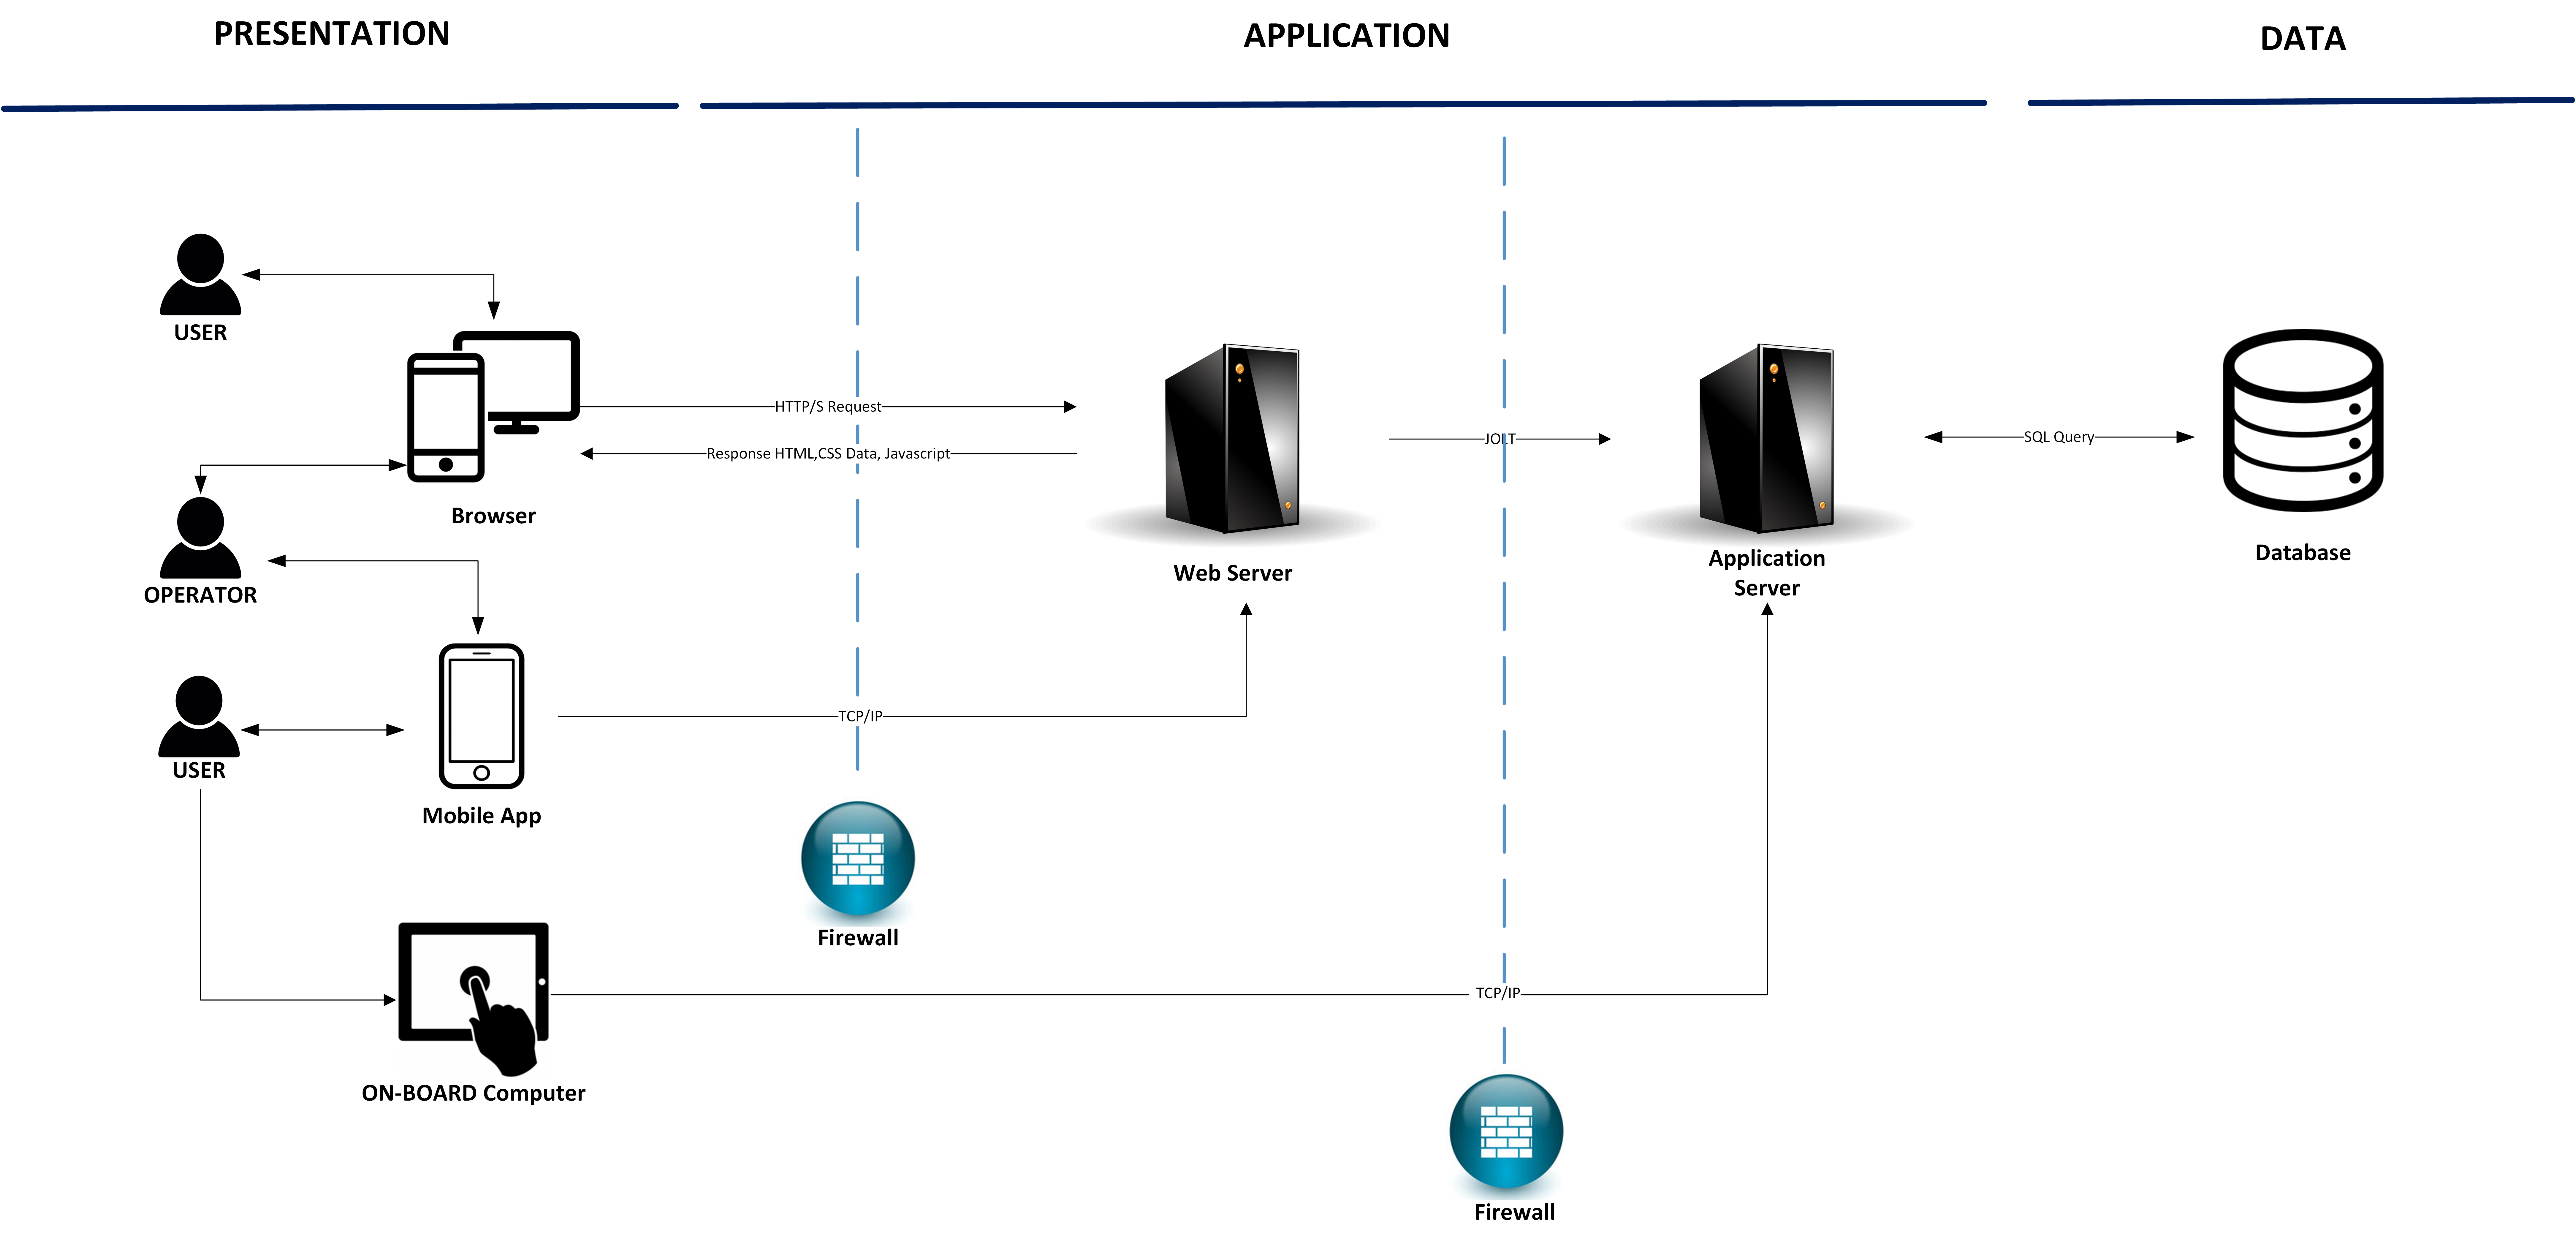
\includegraphics[width=15cm, height=8cm]{architecture} 

\vspace{0.5cm}

\textbf{Mapping between layers and tiers}
\begin{description}
\item PRESENTATION TIER: consists on the web browser, the mobile app and the on-board computers of the cars. These are light clients, which only correspond to the presentation layers. The web browser and mobile app communicate to the web server, sending HTTP/S requests and receiving the HTML, CSS, JAVASCRIPT responses;  they need to get through a firewall in order to enhance security. The on-board computers directly communicate with the application server, since the security is already granted by the card ID recognition, at the moment when the car is unlocked.
\item APPLICATION TIER: consists on a web server and an application server; the web server (Apache HTTP server) processes the HTTP/S requests coming from the clients, elaborates the web pages and generates dynamic contents. The application server contains all the business logics. It receives its inputs from the web server and the on-board computers, and does all the needed computation in order to generate the dynamic pages and  provide them 
to the clients. It can communicate to the Oracle database. There is a firewall between the web server and the application server.
\item DATA TIER:  it consists on the database, which contains all the needed information about users, cars, reservations, operators et al. , which can be accessed by the application server via sql queries.


\end{description}







\subsection{Component View}  %2.2) COMPONENTS
\subsubsection{High level component view} %2.2.1) HL COMPONENTS
The figure below shows the main high level components of the application and the interaction among them.
\vspace{1.5cm}


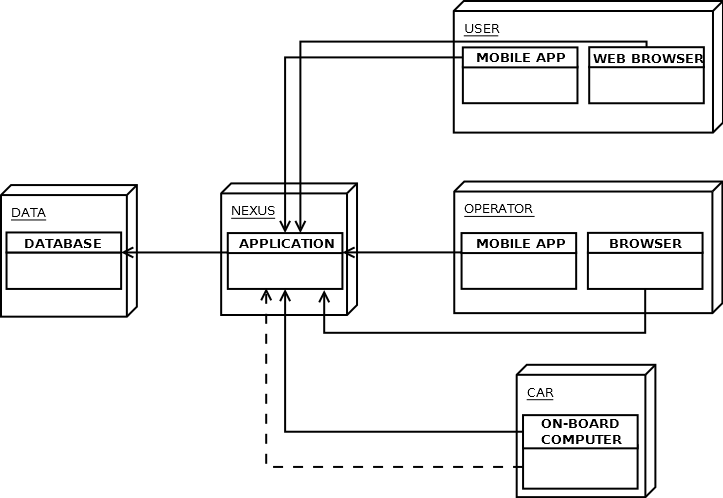
\includegraphics[width=15cm, height=10cm]{HLComponent} 


\vspace{1.5cm}
The nexus is where the core of the application is allocated, which contains all the business logics. It needs to communicate with several other components as follows.




\begin {itemize}
\item The User can establish a connection with the nexus via the mobile app and web browser logging in and requesting the information about the cars he can reserve. This is a synchronous communication, since the user needs to wait the response from the nexus, before going on asking for a car reservation, etc. 
\item The operators can establish an synchronous communication with the nexus in order to take care of cars: they can request to the nexus the list of cars and their information logging in, and, once the nexus provided it to them, they can choose a car to take care of and click on the "Operate" button associate to that car, so that the nexus can update the list, and the same when the issue is resolved.

\item The on-board computer of the cars has an asynchronous communication with the nexus, in order to provide updated information about the status of all the cars.
\item The on-board computer also needs to establish a synchronous communication with the nexus  when users want to unlock the cars they reserved, start and end their ride.
\item The nexus also needs to store and access all the information about users, operators, rides, cars positions and status on the database.
\end{itemize}

\break
\subsubsection{Component View}
 %2.2.3)COMPONENT VIEW
 
\vspace{0.5cm}

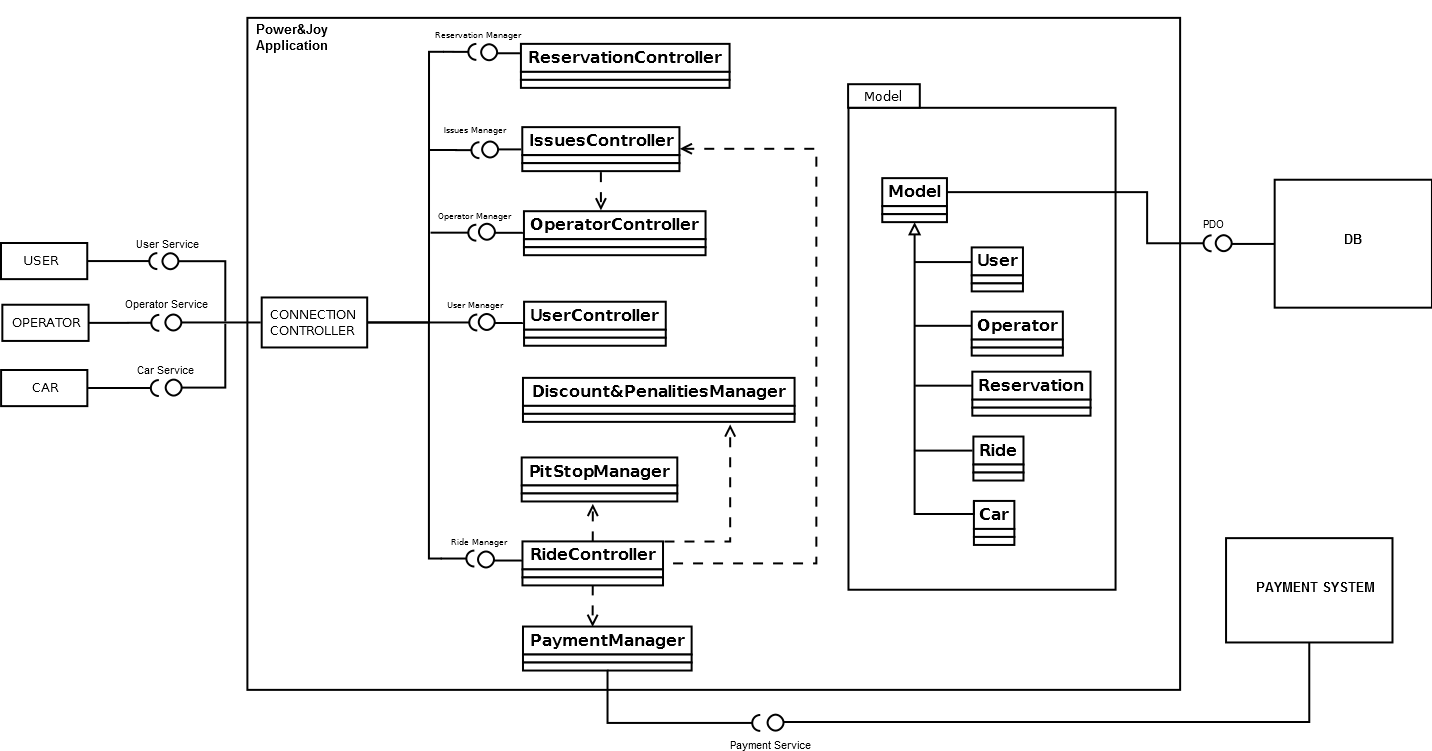
\includegraphics[scale=0.3]{component} 

\vspace{0.5cm}
\begin {itemize}
\item Reservation Controller: manages reservation requests
\item Issues Controller:  supervises  and updates car statuses in case issues occur during a ride
\item Operator Controller: manages operators information and activities
\item User Controller: manages users information 
\item Discounts\&Penalties Manager : computes the final price of the rides  taking into account the information acquired from the on-board computer and the discounts and penalties rules
\item PitStop Manager : manages the duration and fees of the pitstops during the rides 
\item RideManager : manages all the ride information
\item PaymentManager : extracts the information about the rides and the users (credit card number and final price) and sends them to the payment system
\item Connection Controller: dispatches the incoming requests to the appropriate Controller, which will then do the needed work as described above

\end{itemize}


\subsection{Deployment View}  %2.3) DEPLOYMENT
\vspace{4cm}

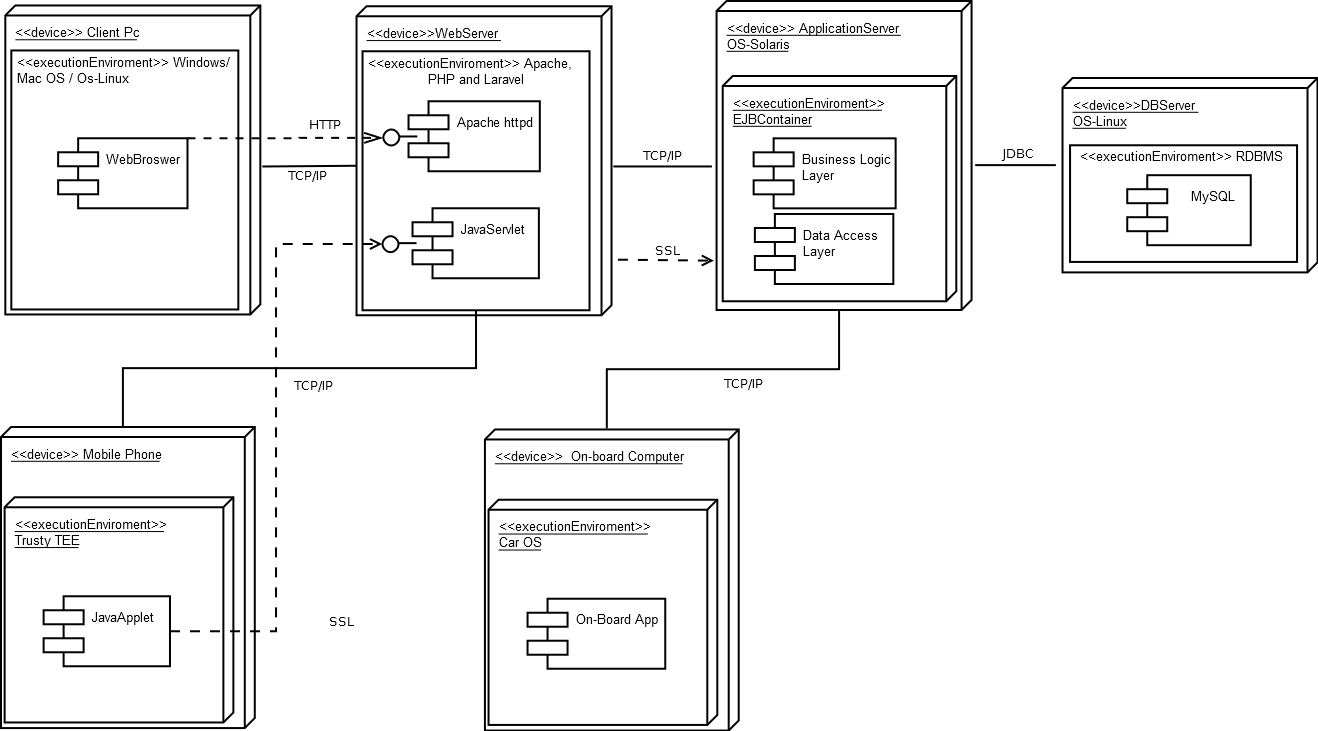
\includegraphics[scale=0.3]{deployment} 





\subsection{Runtime View} %2.4) RUNTIME
%SEQUENCE

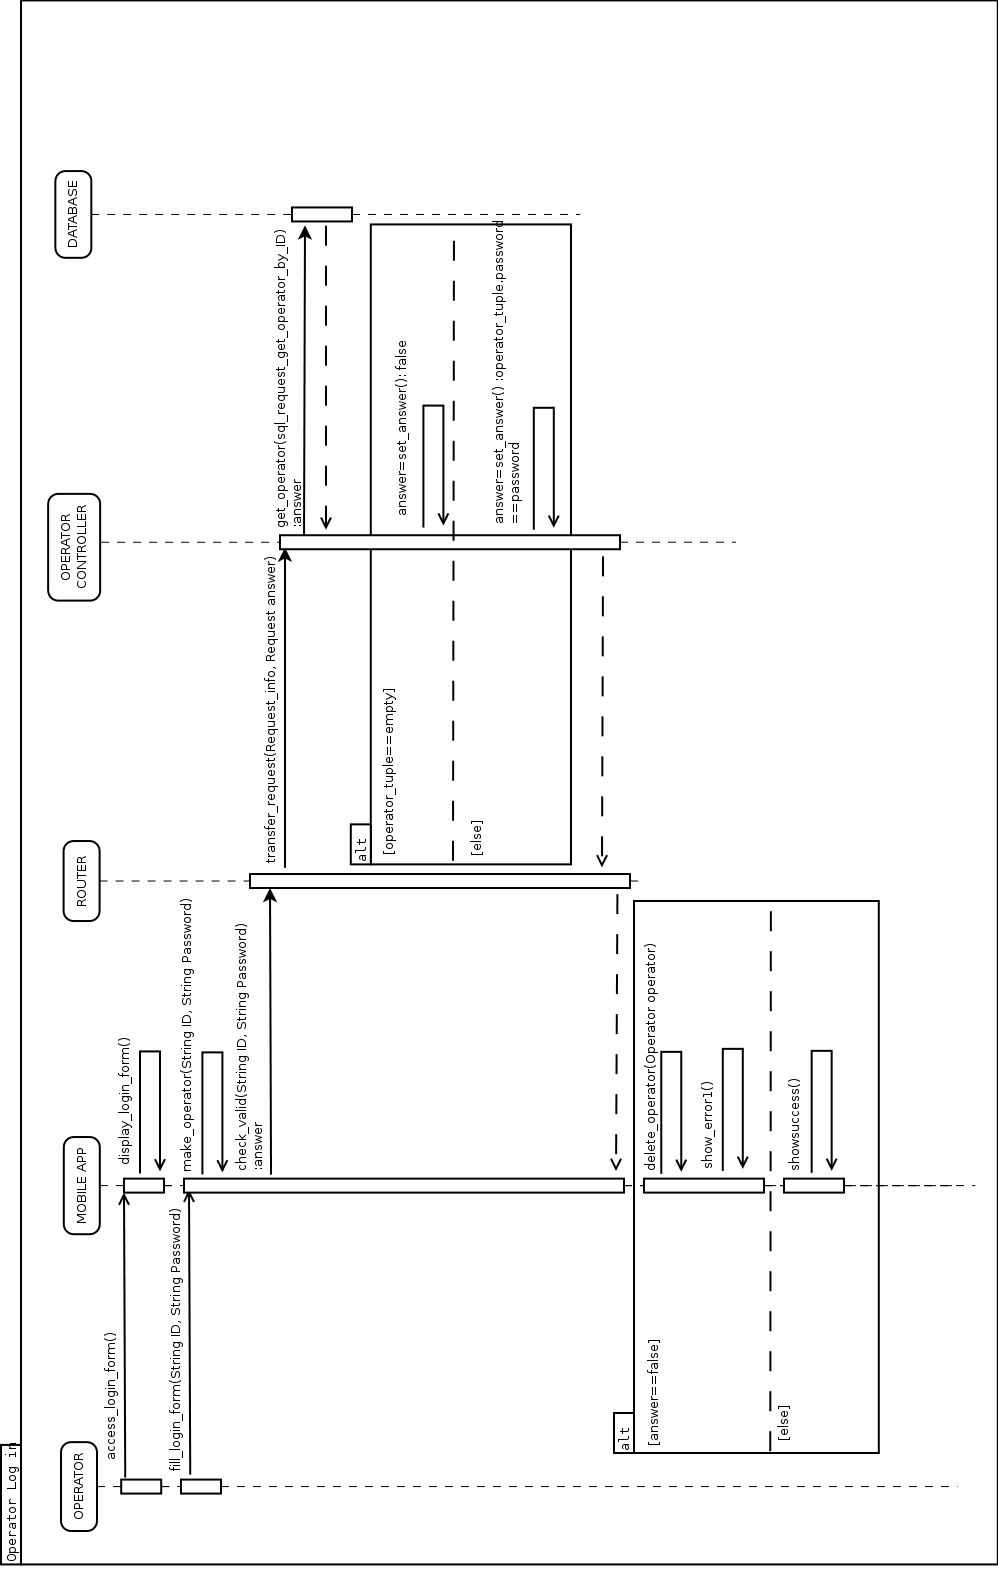
\includegraphics[scale=0.4]{seq1_login} 
\newpage
\textbf{Sequence Diagram 1: Operator Login}
\break
The above diagram shows how an operator can log into the system. In order to do that, he has to be registered first. The operator accesses the login page from his mobile app and inputs his credentials (an ID and a password). The mobile app transfers this request to the operator controller, that checks that there is a tuple corresponding to that operator into the database. If there is one, then the operator controller sets the answer to ''true'' only if the password that the operator inserted matches with the one saved on the tuple. The mobile app receives the answer and shows the operator home page only if the answer is true. Otherwise it shows an instance of error1 (inserted credentials not valid). \\
The router that appears as an actor sums up the actual device which takes care to send the request through the network to the application server and the connection controller, that receives the request and pushes it to the right controller component in the application.\\
The log in (as well as all other operations) via the web browser is analogous to the one via mobile app.\\
Log in for the users involves the same operations, with the User Controller instead of the Operator one.



\newpage
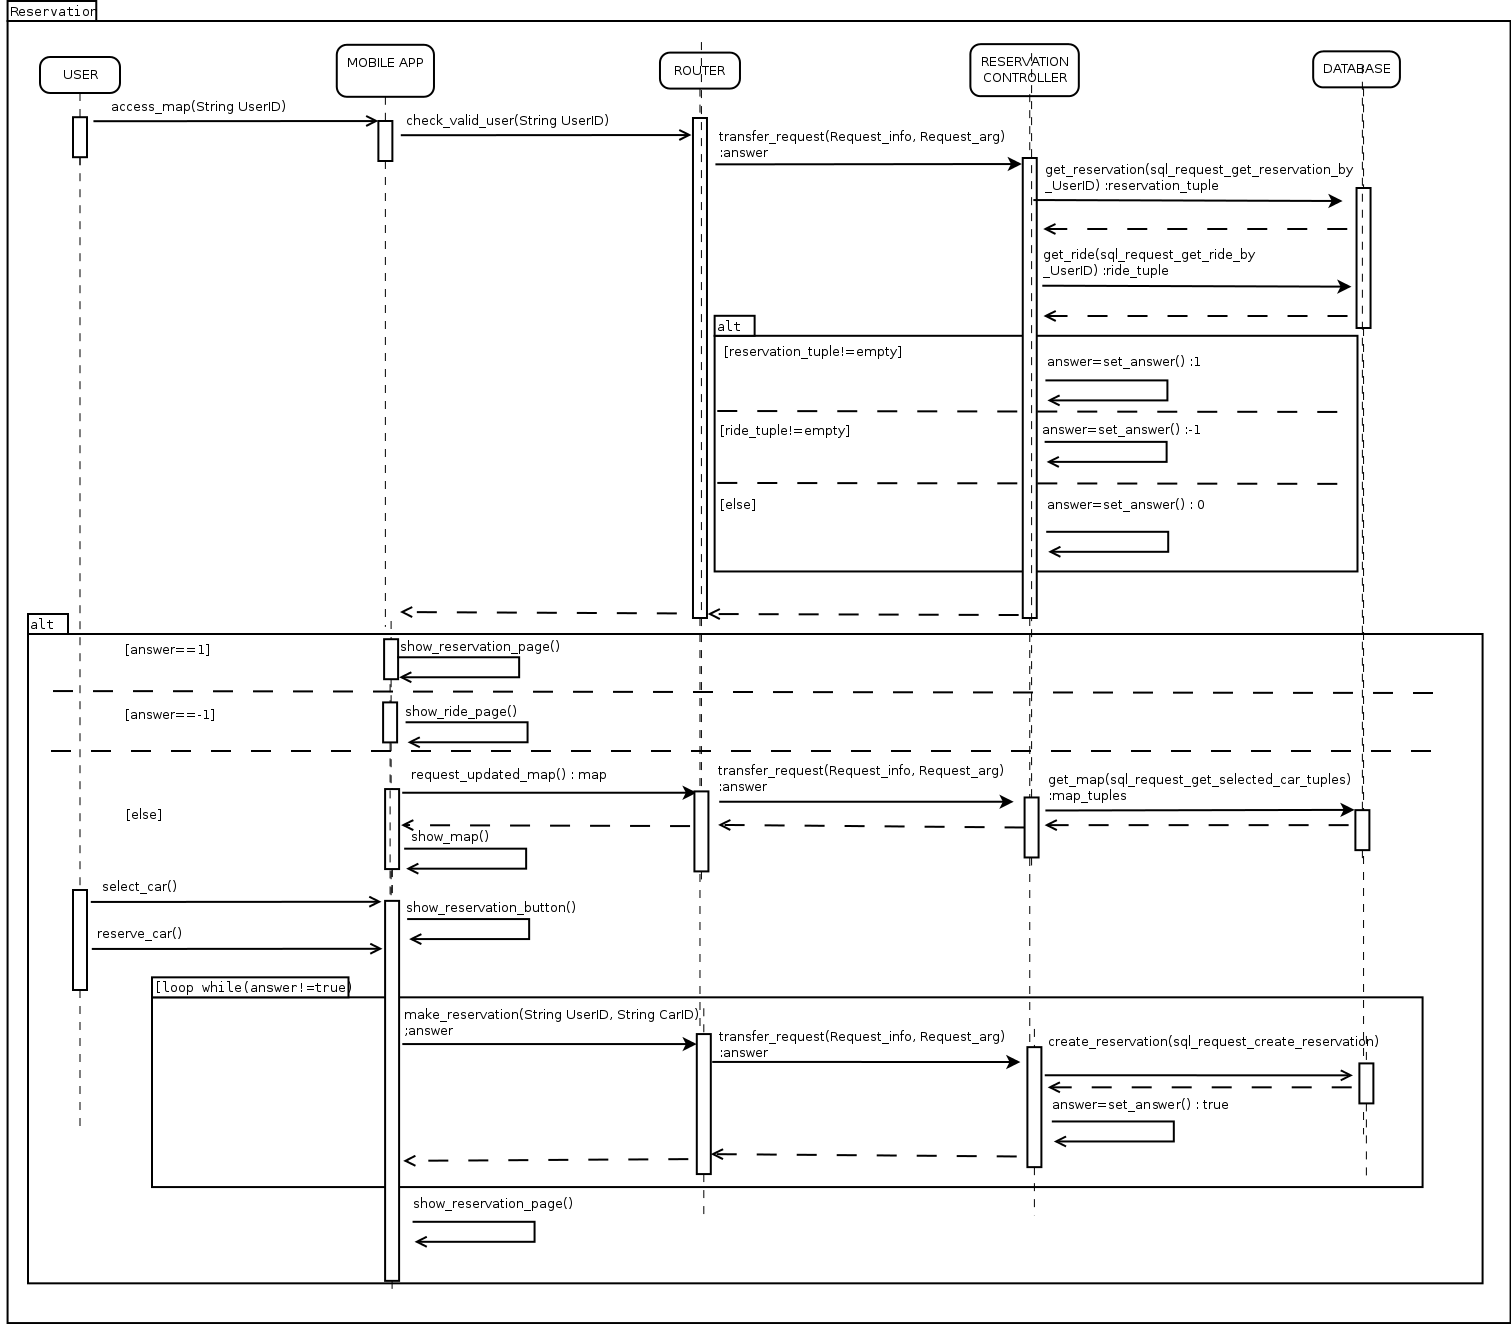
\includegraphics[scale=0.3]{seq2_reservation} 
\newpage
\textbf{Sequence Diagram 2: User reserves a car}
\break
The above diagram shows the actions performed in order to let a user reserve a car. \\
The user has to be registered and have successfully inserted his credentials to log in. Once he submits them (assuming they have been already checked as valid) , the mobile app sends a request to show the map to localize the cars. This request arrives to the Reservation Controller, that first needs to check if the user has already an ongoing reservation or ride. It interrogates the database, and sets the answer to a value that distinguishes the following three cases:
\begin{enumerate}
\item A valid reservation tuple (which means one associated to a reservation which is not expired yet) associated to the user is found; Then answer is set to ''1'', and the user is redirected to the reservation page corresponding to the reservation he already performed
\item A ride tuple associated to the user is found: this means that the user is already performing a ride; then the answer is set to ''-1'' and an instance of error2 (already on a ride) is showed and the user is not redirected anywhere until the ride ends.
\item Neither a valid reservation or ride associated to the user is found; then the answer is set to 0, and the mobile app shows the map with the cars . 
\end{enumerate} 
The third case is further exploited, in order to show how a user can actually reserve a car; he selects a car, and the app shows the reservation button; the user taps on that button and a request of a new reservation is sent to the reservation controller, which creates a new instance of reservation and updates the database. The user is then redirected to the reservation page, where he can see all the reservation details such as the carID, the timer, the car position ecc.


\newpage
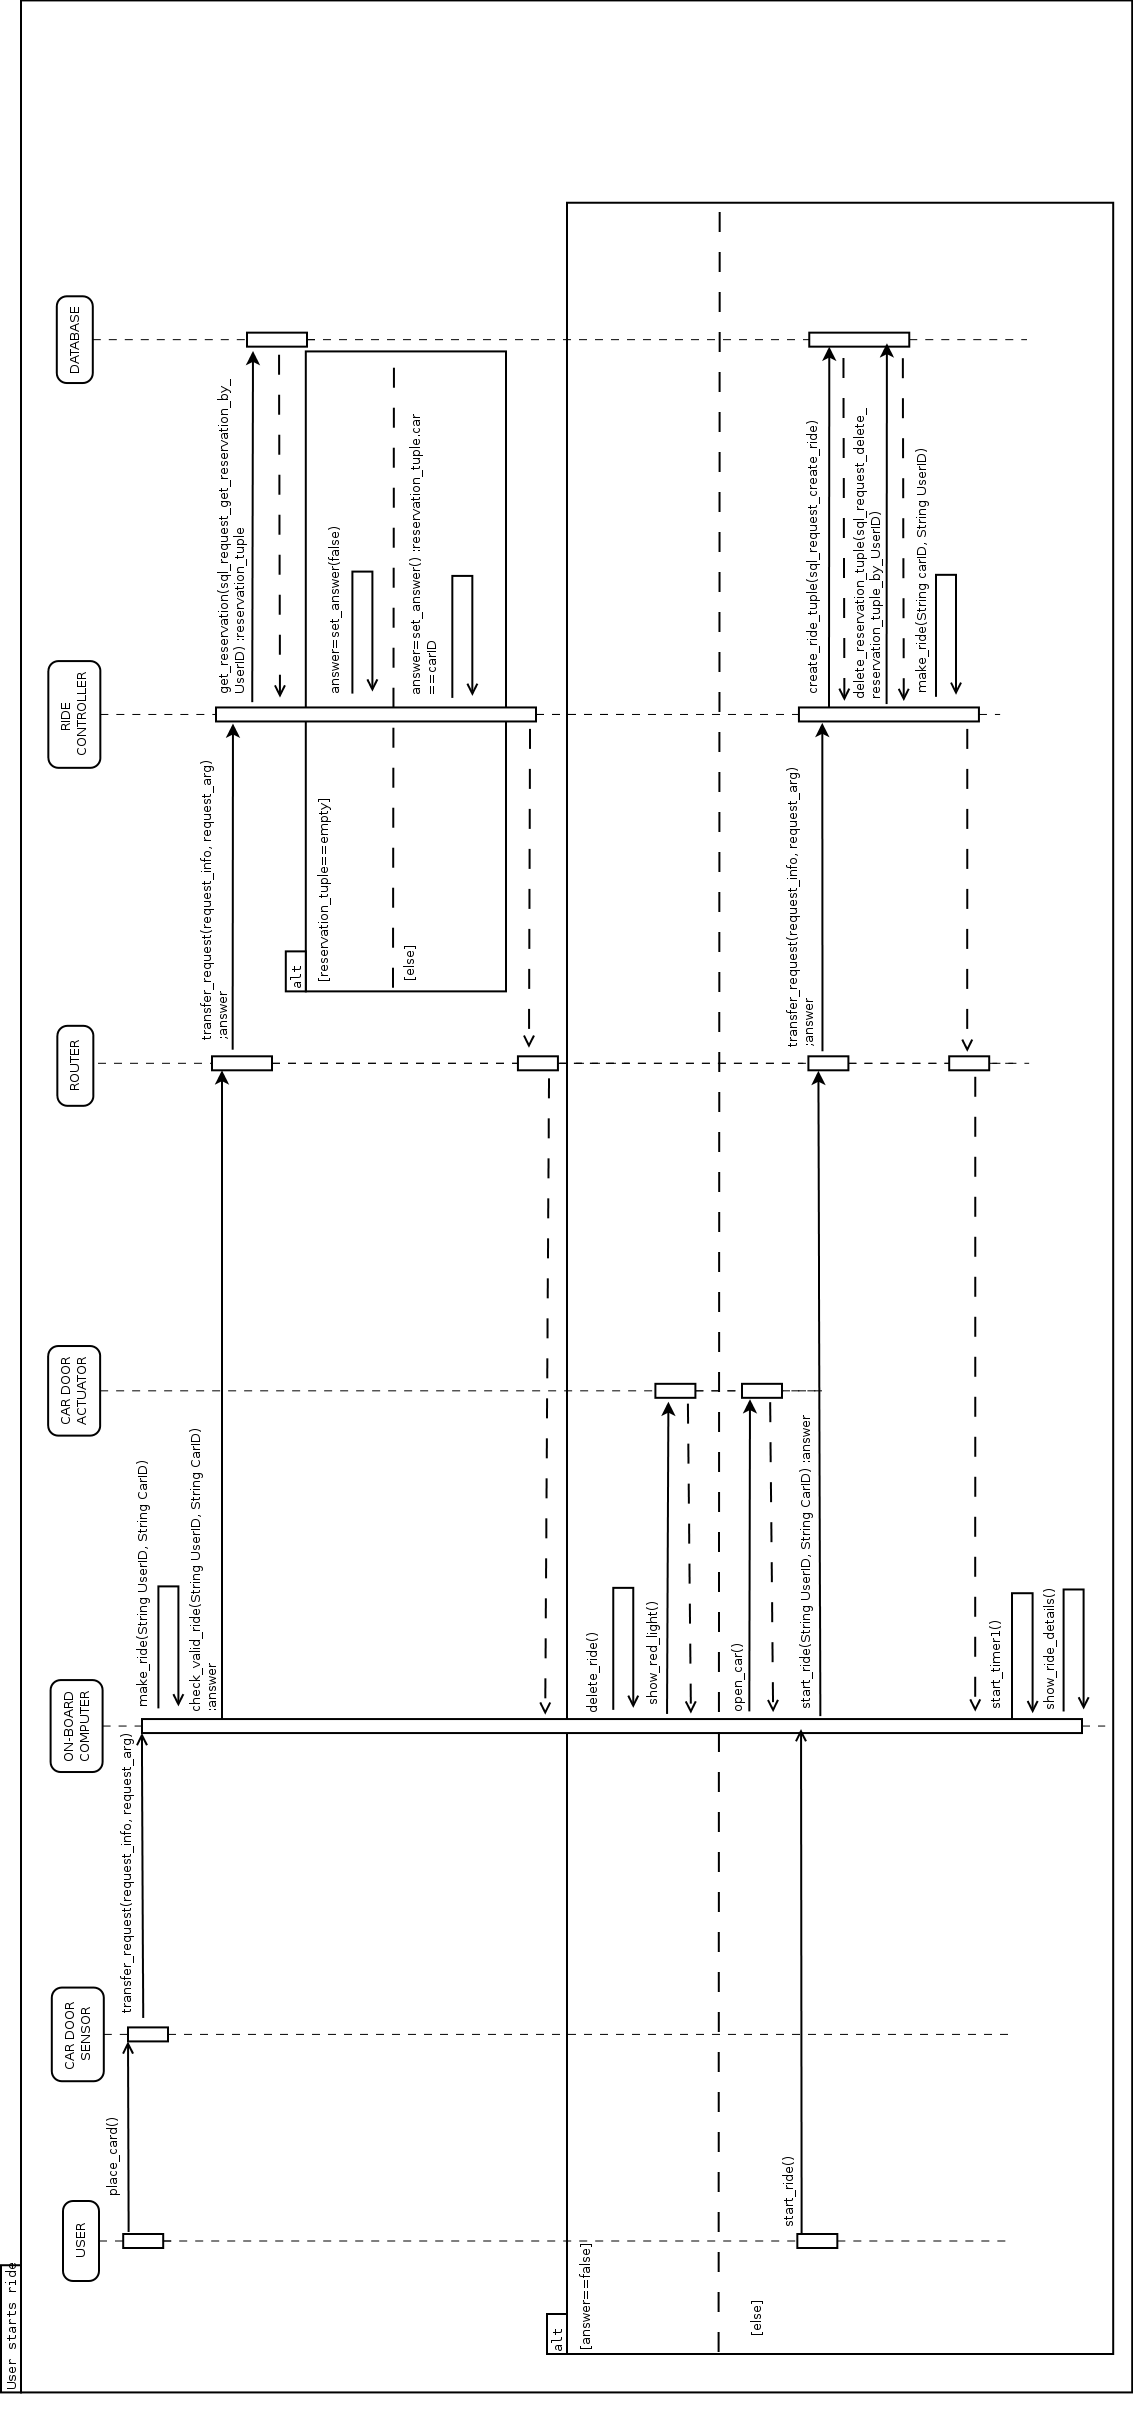
\includegraphics[scale=0.25]{seq3_start_ride} 
\newpage
\textbf{Sequence Diagram 3: User starts a ride}
\break
We already said, back in RASD, how the car should be provided with an appropriate system of its own, which means it has to be equipped with all the needed sensors and actuators communicating with the on-board computer, which can send requests to the application server in order to perform all the operations to let the user ride the car.\\
The above diagram describes the start of the ride, which is requested by the user by placing its contact-less card on the door sensor. Then a request is sent to the Ride controller, that checks that the user has a valid on-going reservation. The answer is set to ''true''only if a valid tuple is found and the carID on the reservation tuple matcher the one of the car that the user is trying to unlock. If that happens, the doors are unlocked, otherwise, a red light is shown and the doors remain locked.
If the user manages to correctly unlock the car and starting the ride tapping on the ''START RIDE'' button on the on-board computer, then the ride controller updates the database removing the reservation tuple and adding a ride one, and creates a new instance of ride. Once these operations are correctly performed, the on-board computer starts the timer, to store the information about the ride length, which is then sent to the application server (once the ride terminates, which is not shown in the diagram) to perform the payment 

\newpage
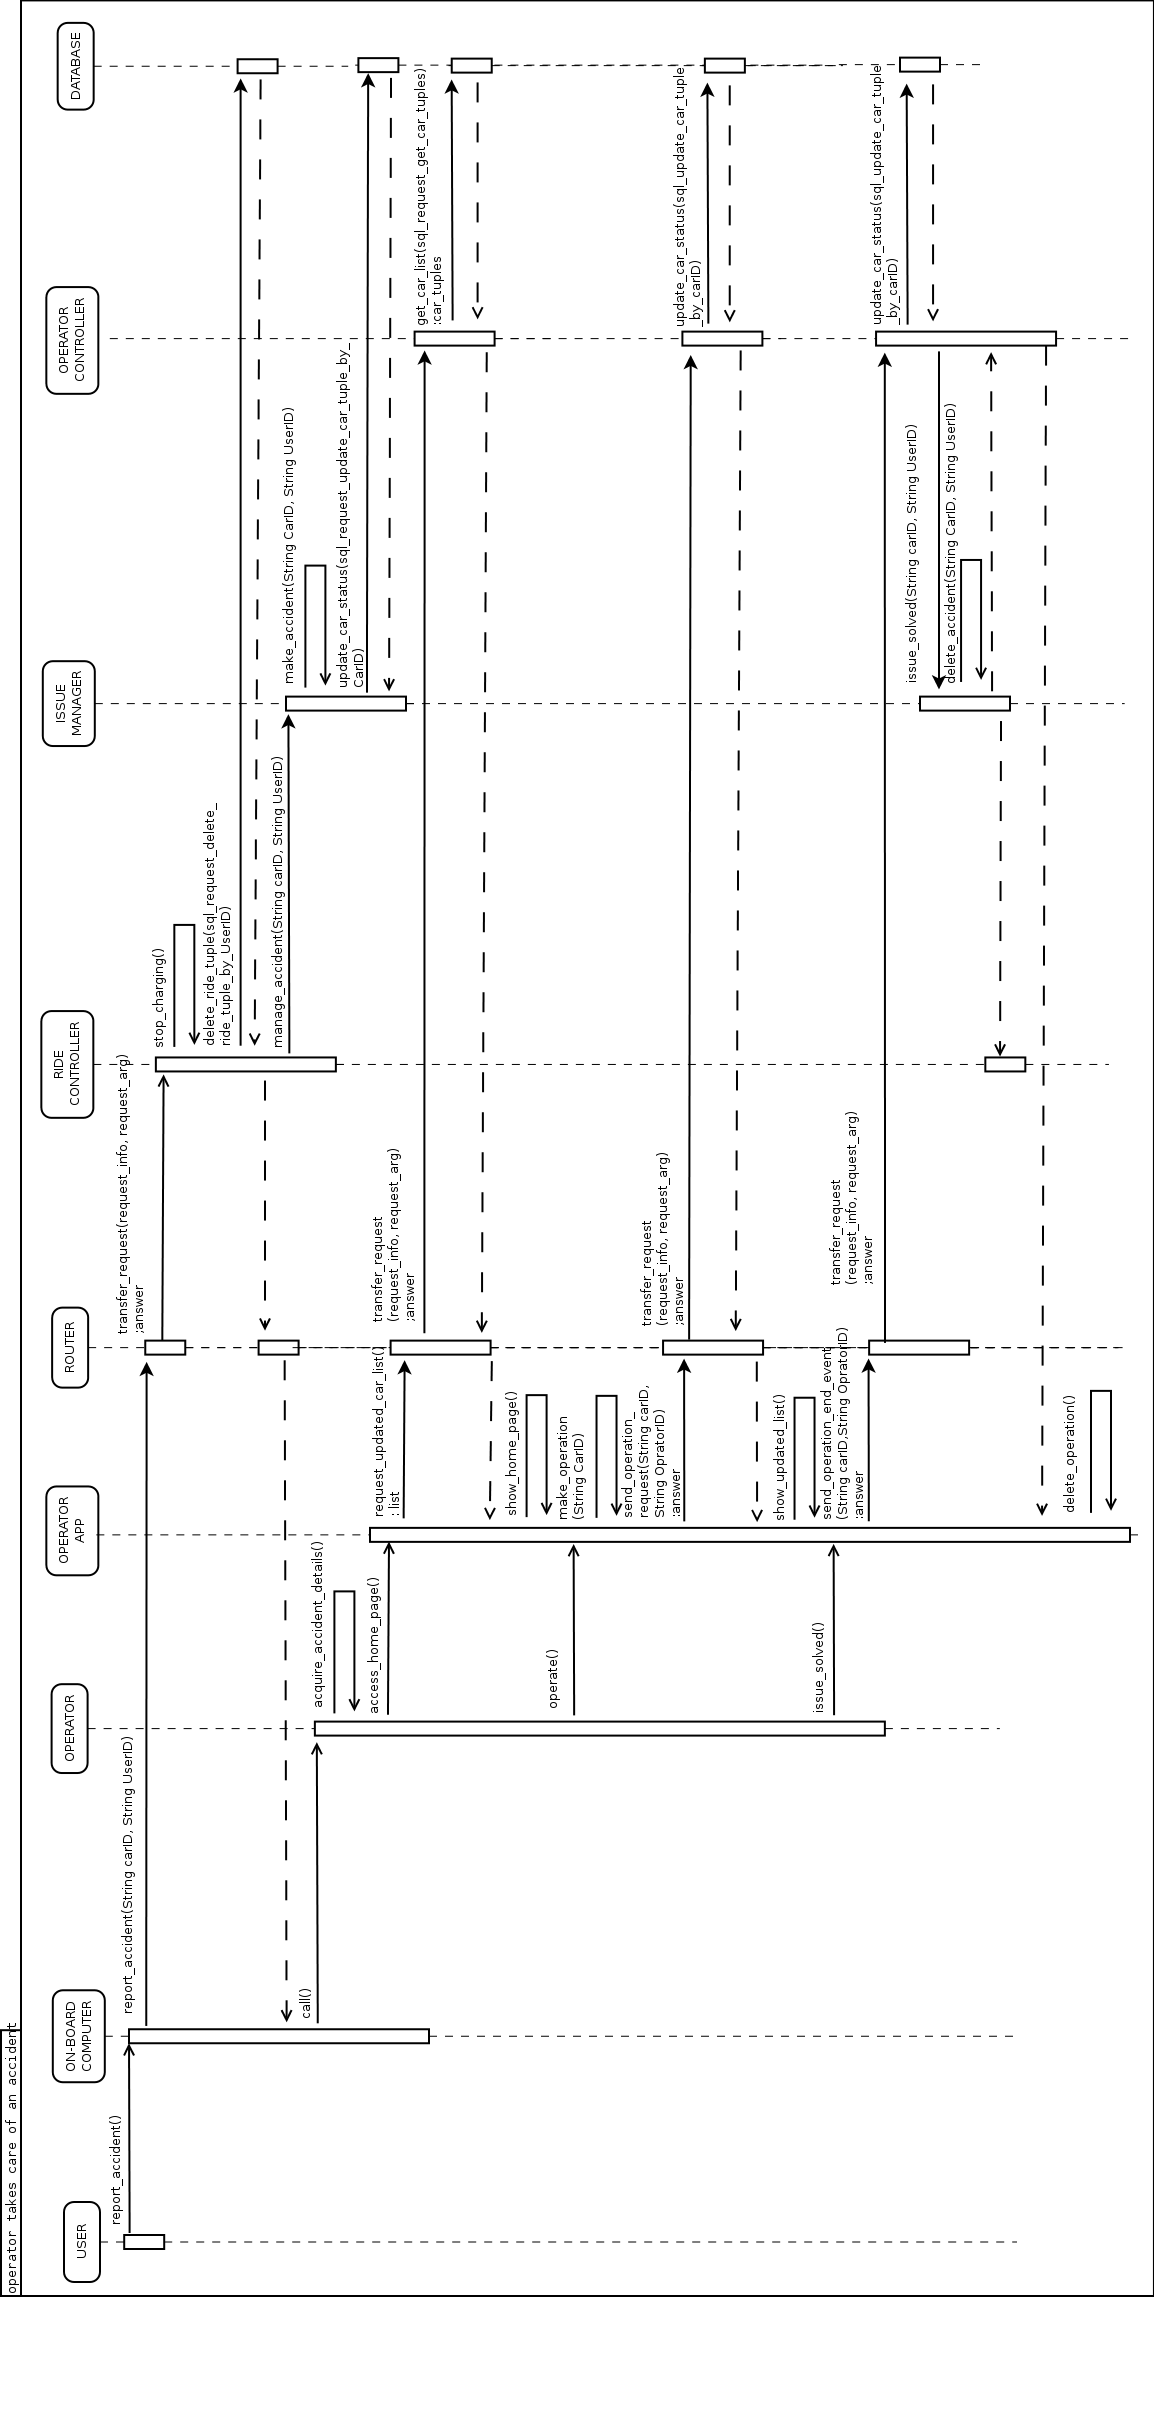
\includegraphics[scale=0.25]{seq4_accident} 
\newpage
\textbf{Sequence Diagram 4: Accident}
\break
The above diagram shows the actions performed in case an accident occurs. It is signaled by the user tapping a dedicated button on the on-board computer. The on-board computer then sends a request to the ride controller, which terminates the ride. It stops charging the user and deletes the ride tuple on the database, but saves locally the information about the ride itself in order to lately perform the payment. It also sends a request to the issue controller, which creates an instance of accident and updates the car status on the database, in order to let all the operators know about what happened. Once all these operations have been correctly performed, the on-board computer makes a call to an operator, which acquires the accident details from the user. Once he is satisfied, he accesses its home page (logging in as described in Sequence Diagram 1) requesting the updated list to the operator controller, and looks for the row on the list corresponding to the car involved in the accident. He then taps on the ''OPERATE'' button, and the mobile app creates an instance of operation and sends a request to the operator controller in order to update the car status informing all other operators that issue is already being taken care of. Once the operator provided assistance to the user, he informs the operator controller tapping on the ''ISSUE SOLVED'' button. The operator controller updates the car tuple once again and informs the issue controller that the issue has been solved. The issue manager deletes the accident instance, and the operator mobile app deletes the operation instance.


\newpage

\subsection{Component Interfaces} %2.5) INTERFACES
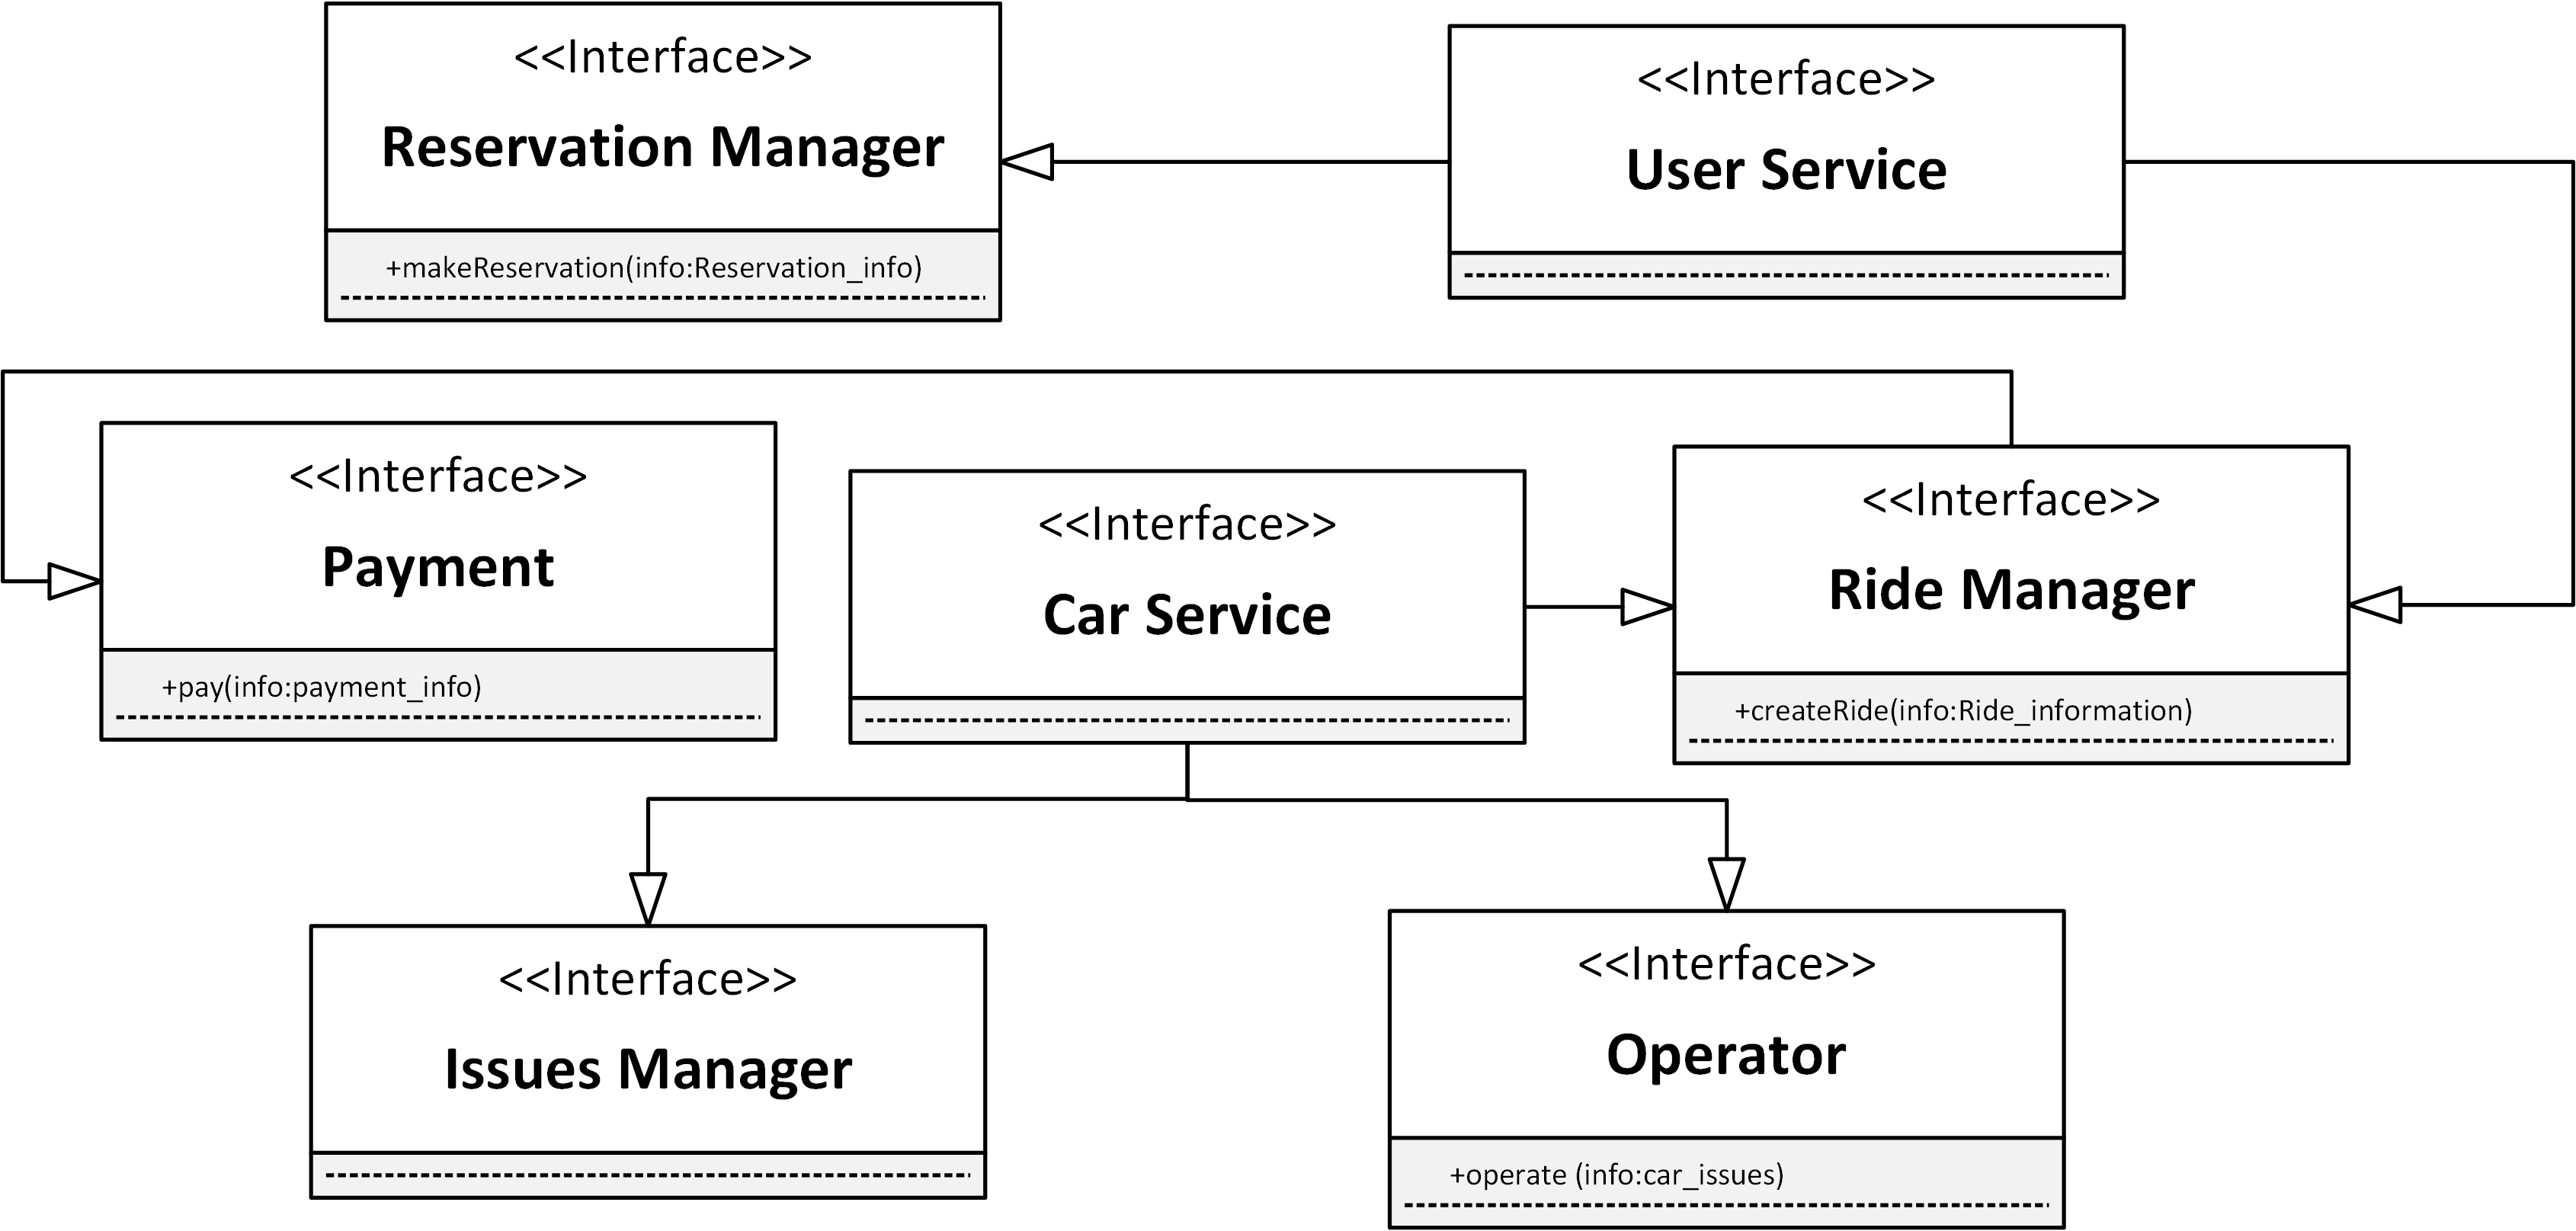
\includegraphics[scale=0.7]{interface} 

\subsection{Selected Architectural Styles and Patterns} %2.6) SSASP 
\subsubsection{Overall Architecture}
Our application will be divided into 3 tiers:\\
\begin{enumerate}
\item Presentation tier (thin clients )
\item Application tier (contains all the business logic)
\item Data tier (database to store all information)
\end{enumerate}
\subsubsection{Protocols}
Our tiers are connected through network and exchange data with the following protocols.
\vspace{1cm}
\\

\textbf{PHP}(Hypertext Preprocessor) : used to generate dynamic web pages\break\break

\textbf{PDO}(PHP Data Objects): used by the Business logics to communicate with the Data layer. \break\break

\textbf{HTTPS} (Hyper Text Transfer Protocol over Secure Socket Layer): application layer protocol used for sharing information in a safe way across the World Wide Web . It's a typical protocol used in a client-server architecture\break\break

\textbf{TCP/IP}(Internet Protocol Suite) : provides and-to-end data communication specifying how data should be packetized, addressed, transmitted, routed and received.\break\break

\textbf{SSL}(Secure Socket Layer): cryptographic protocol used to provide communication security over a computer network. Its aim is to provide privacy and data integrity between two communicating computer applications\break\break

\textbf{JDBC}(Java DataBase Connectivity): application programming interface (API) for the programming language Java, which defines how a client may access a database. It provides methods to query and update data in a database, and is oriented towards relational databases \break\break

\textbf{Trusty TEE}(Trusted Excecution Environment) that consists of:
\begin{itemize}
\item An operating system (the Trusty OS) that runs on a processor intended to provide a TEE
\item Drivers for the Android kernel (Linux) to facilitate communication with applications running under the Trusty OS
\item A set of libraries for Android systems software to facilitate communication with trusted applications executed within the Trusty OS using the kernel drivers

\end{itemize} 
\vspace{1cm}



\subsubsection{Design Patterns}

\textbf{MVC}(Model View Controller) comes in the form of the Laravel PHP framework as well as the internal component structure of the software components running on the application server\\
\textbf{Client-Server}  is used to partition the tasks between the provider of the service (server) and the service requesters (web browser and mobile application used by users and operators and the on-board computer). This is useful because of its centralized structure that allows us to have thin client , for accessibility of the resources remotely allocated, and security  thanks to access rights to the data, which is all stored in the same place


\subsection{Other Design Decisions} %2.7) ODD
We also decided to integrate our web application and our mobile applications with a map service.

\section{Algorithm Design} %3) ALGORITHM
\begin{lstlisting}
import java.util.Calendar;
import java.util.logging.Level;
import java.util.logging.Logger;

import it.polimi.ingsw.ps09.net.Server;

public class ReservationController {
	 //Calendar cal = Calendar.getInstance();
	private static final Logger LOGGER = 
	Logger.getLogger(ReservationController.class.getName());
    
	
	public ArrayList<Reservation> reservationArray = 
	new ArrayList<Reservation>();
	
	public Reservation MakeReservation (User user, Car car, Calendar cal){
		if(model.user.getUsers().contains(user)){
		String userId = user.getId();
		String carId = car.getId();
	Reservation res = new Reservation(userId, carId, cal, true);
	reservationArray.add(res);
	return res;
		}
		else 
			LOGGER.log(Level.INFO,"You have to 
			register into the system");
		return null;
	}
	public boolean valid (Reservation res) {
		Calendar now = Calendar.getInstance();
		int hourNow = now.get(Calender.HOUR_OF_DAY)*60 ;
		int minuteNow  = now.get(Calender.MINUTE);
		int timeCurrent = hourNow+ minuteNow;
		
		int hour = res.getCalender().get(Calender.HOUR_OF_DAY)*60;
		int minute  = res.getCalender().get(Calender.MINUTE);
		int time = hour + minute;
		
		if(timeCurrent > (time+60)){
			return false;
		}else{
			return true;
		}	
	}
	
	public void cancelReservation(res){
		reservationArray.remove(res);
	}
	
	public void reservedForSixtyMinutes(Reservation res){
		Calendar now = Calendar.getInstance();
		int hourNow = now.get(Calender.HOUR_OF_DAY)*60 ;
		int minuteNow  = now.get(Calender.MINUTE);
		int timeCurrent = hourNow+ minuteNow;
		
		int hour = res.getCalender().get(Calender.HOUR_OF_DAY)*60;
		int minute  = res.getCalender().get(Calender.MINUTE);
		int time = hour + minute;
		
		while(timeCurrent<time){
			now.getInstance();
			hourNow = now.get(Calender.HOUR_OF_DAY)*60 ;
			minuteNow  = now.get(Calender.MINUTE);
			timeCurrent = hourNow+ minuteNow;
			if (rideStart==true){
				break;
			}
		}
		if (rideStart==false){
			Reservation resRemoved = 
			reservationArray.remove(res);
		}
		
	}
}

\end{lstlisting}
\newpage

\begin{lstlisting}
import java.util.Calendar;
import java.util.logging.Level;
import java.util.logging.Logger;

public class RideController {

	private static final Logger LOGGER = 
	Logger.getLogger(RideController.class.getName());
	
public ArrayList<Ride> rideArray = new ArrayList<Ride>();
	
	public Ride CreateRide (String rideId, User user, 
	Car car, Calendar cal, 
	TypeIssue type, Int duration, Double cost){
		if(model.user.getUsers().contains(user)){
		String userId = user.getId();
		String carId = car.getId();
	Ride ride = new Ride(rideId, userId, carId, cal,type, 
	duration, cost, true);
	/* 
	 * type= noIssues
	 * duration = 0
	 * cost = 0
	 * the ride is valid =  true
	 */
	rideArray.add(ride);
	return ride;
		}
		else 
			LOGGER.log(Level.INFO,"You did not 
			register into the system");
		return null;
	}
	
	public void issuesRide (Ride ride){
		TypeIssue issue = car.getStatus();
		ride.setStatus(issue);
		if(issue==ACCIDENT){
			endRide(ride);
		}
		
	}
	
	public double endRide (Ride ride){
		int duration = getDuration(ride);
		int passengers = getPassengers(ride);
		ride.setDuration(duration);
		ride.setPassengers(passengers);
		double finalCost = computeFinalCost(passengers,duration);
		rideArray.remove(ride);
		return finalCost;
	}
	
	public int getDuration(Ride ride){
		Calendar now = Calendar.getInstance();
		int hourNow = now.get(Calender.HOUR_OF_DAY)*60 ;
		int minuteNow  = now.get(Calender.MINUTE);
		int timeCurrent = hourNow+ minuteNow;
		
		int hour = ride.getCalender().get(Calender.HOUR_OF_DAY)*60;
		int minute  = ride.getCalender().get(Calender.MINUTE);
		int time = hour + minute;
		
		int duration = timeCurrent - time;
		
		return duration;
	}
	
	public double computeFinalCost (int passengers,int duration){
		double firstCost = duration * 0.25;
		int discount = 0;
		int penalties = 0;
		if(car.getLevelCharge() >= 50){
			discount+= 20;
		}else if (car.getLevelCharge()< 20){
			penalties+=30;
		}
		
		if(car.getThreekmAway()){
			penalties+= 30;
		}
		
		if(passengers>=2){
			discount+=10;
		}
		
		if (car.getPluggedIn()){
			discount+=30;
		}
		double finalCost= 0;
		if(discount>0){
			finalCost = (firstCost - ((firstCost*discount)/100));
		}
		 if (penalties>0){
			finalCost = (firstCost + ((firstCost*penalties)/100));
		}
		return finalCost;
	}
	
	
}
\end{lstlisting}

\section{User Interface Design} %4) UX
\subsection{Mockups}%4.1) MOCKUPS
We have already done mockups in RASD in section 3.3\break
\newpage
\subsection{UX diagrams} %4.2) UX
The following UX diagrams show the main interactions between the system and the users and operators\break


\includegraphics[width=15cm, height=12cm]{UxRegistrationReservation} \break
 



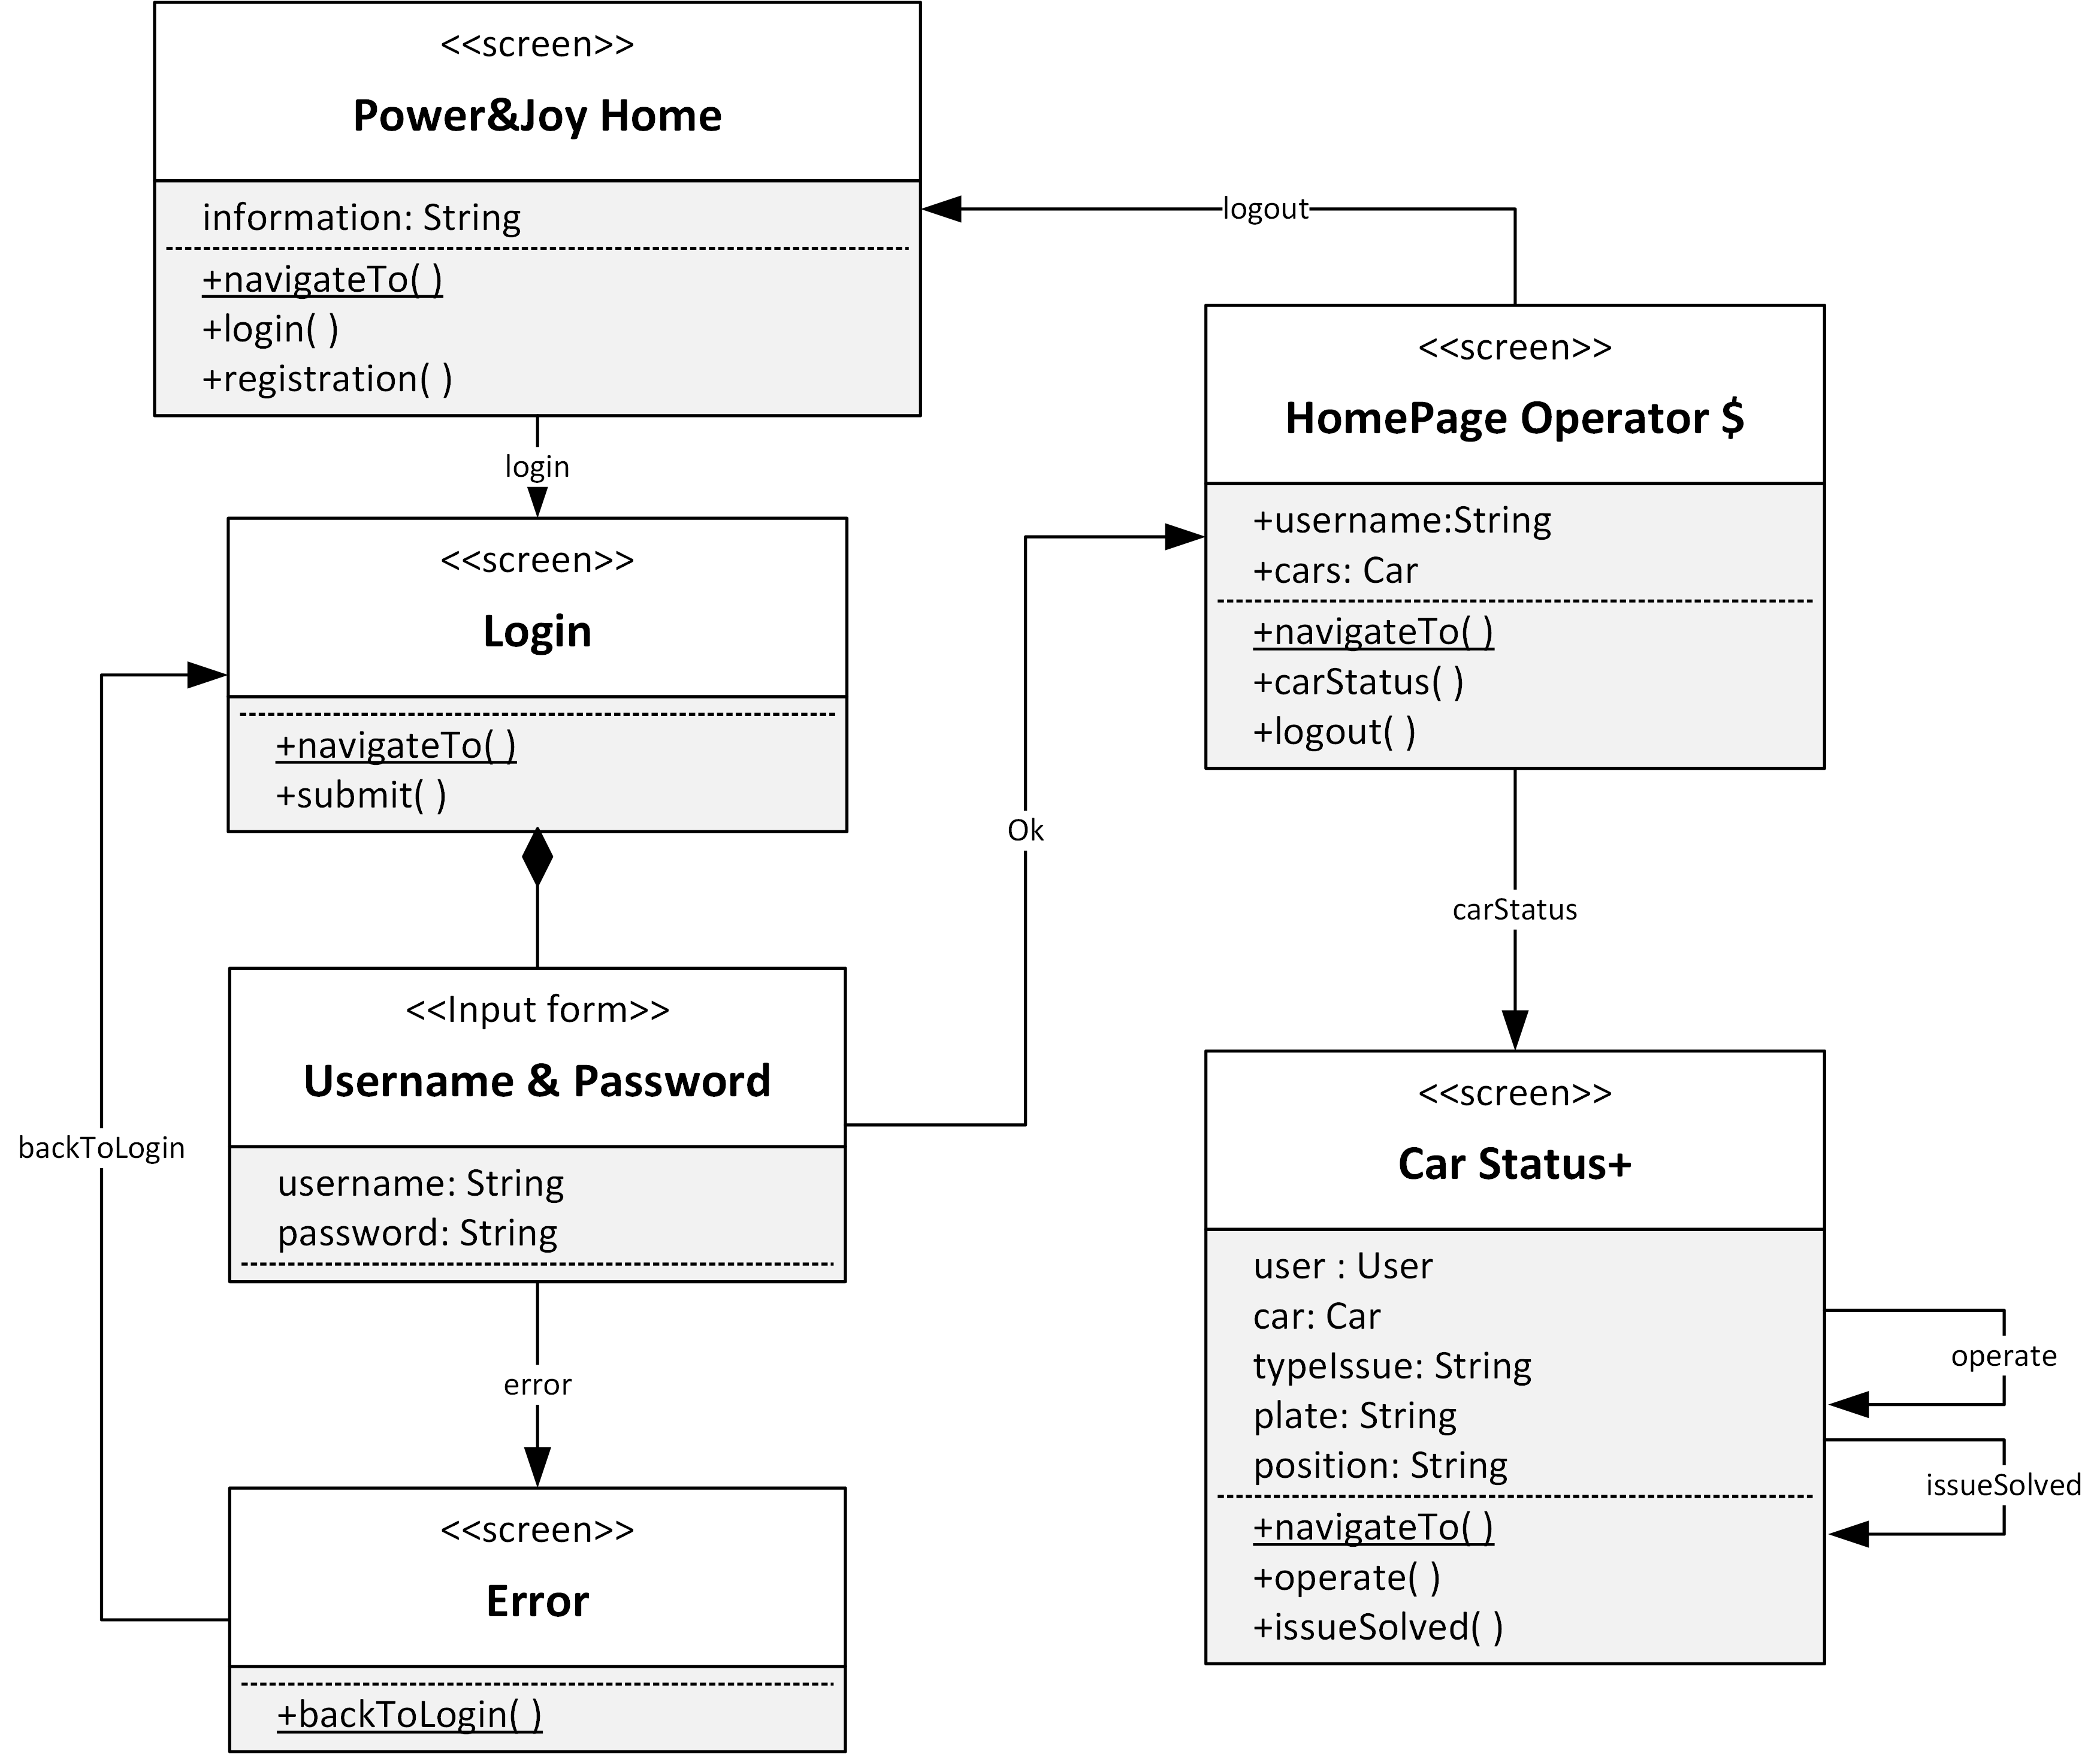
\includegraphics[width=15cm, height=12cm]{operatorux} 
\newpage
\subsection{BCE diagram}
The BCE diagram is used to describe how the requests from the users and operators are managed by the application, accordingly to the MVC design pattern

\vspace{1cm}
\includegraphics[width=15cm, height=12cm]{BCE} 
\vspace{1cm}
\newpage


\section{Requirement Traceability} %5) REQ TRACEABILITY
This section will describe how the application components are linked to the requirements in the RASD document.
\begin{description}


\item [G1] The system shall allow users to register via the web or mobile app by inserting all the required information
\begin{itemize}
\item User Controller
\item Connection Controller
\item Database
\end{itemize}
\item [G2] The system shall allow users to log in
\begin{itemize}
\item UserController
\item ConnectionController
\item Database
\end{itemize}
\item [G3] The system shall allow users to see the positions of all the available cars on a map
\begin{itemize}
\item Reservation Controller
\item Connection Controller
\item Database
\end{itemize}
\item [G4] The system shall allow users to make a reservation for an available car
\begin{itemize}
\item Reservation Controller
\item Connection Controller
\item Database
\end{itemize}
\item [G5] The system shall allow users who reserved a car to cancel the reservation
\begin{itemize}
\item Reservation Controller
\item Connection Controller
\item Database
\end{itemize}
\item [G6] The system shall allow users to unlock the car they reserved
\begin{itemize}
\item Ride Controller
\item Connection Controller
\item Database
\end{itemize}
\item [G7] The system shall allow users to start the ride
\begin{itemize}
\item Ride Controller
\item Connection Controller
\item Database
\end{itemize}
\item [G8] The System shall allow users to make a pit stop of maximum 60 minutes
\begin{itemize}
\item Ride Controller
\item Connection Controller
\item PitStop Controller
\end{itemize}
\item [G9] The system shall allow users to end the ride 
\begin{itemize}
\item Ride Controller
\item Connection Controller
\end{itemize}
\item [G10] The system shall allow users to communicate if the car they reserved is damaged or issues are found (e.g. dirt, damages, etc.)
\begin{itemize}
\item Ride Controller
\item Connection Controller
\item Issue Manager
\end{itemize}
\item [G11] The system shall compute the price of every ride taking into account discounts and penalties and send it to the system which takes care of the payment
\begin{itemize}
\item Ride Controller
\item Connection Controller
\item Discounts\&Penalities Manager
\end{itemize}
\item [G12] The system shall allow users to report an accident via the on-board computer
\begin{itemize}
\item Ride Controller
\item Connection Controller
\item Issue Manager
\end{itemize}


\item [G13] The system shall allow operators to log into a dedicated area .
\begin{itemize}
\item Operator Controller
\item Connection Controller
\item Database
\end{itemize}
\item [G14] The system shall allow operators to view the updated status and position of every car
\begin{itemize}
\item Operator Controller
\item Connection Controller
\item Database
\end{itemize}
\item [G15] The system shall allow operators to be able to select a car from the list in order to take care of it.
\begin{itemize}
\item Operator Controller
\item Connection Controller
\item Database
\end{itemize}
\item [G16] The system allow an operator who took care of a car to communicate that the issues are resolved to all the other operators
\begin{itemize}
\item Operator Controller
\item Connection Controller
\item Database
\end{itemize}




\end{description}
\newpage
\section{Effort Spent} %6) EFFORT SPENT

\textbf{Joshua Nicolay Ortiz Osorio} \break
\begin{description}
\item 18/11/2016 : 3h
\item 20/11/2016 : 1h30m
\item 23/11/2016 : 3h
\item 25/11/2016 : 2h
\item 26/11/2016 : 1h
\item 30/11/2016 : 30m
\item 05/12/2016 : 2h
\item 08/12/2016 : 3h30m
\item 09/12/2016 : 2h
\item 11/12/2016 : 2h
\end{description}
\vspace{2cm}

\textbf{Michelangelo Medori} \break
\begin{description}
\item 18/11/2016 : 3h
\item 23/11/2016 : 3h
\item 25/11/2016 : 2h
\item 26/11/2016 : 2h30m
\item 27/11/2016 : 4h
\item 08/12/2016 : 3h30m 
\item 10/12/2016 : 2h
\item 11/12/2016 : 2h
\end{description}

\newpage
\section{Used Tools} %7) REFERENCES
The tools we used to create this DD document are:
\begin{itemize}

\item GitHub: for version control
\item Dropbox: to share documents
\item Visio: for Architecture diagram, UX diagrams, BCE diagram and Interfaces diagram
\item DIA: for Sequence, Deployment, Component diagrams
\item Eclipse: for Algorithm view
\item Latex: for writing the document and generating pdf

\end{itemize}
\end{flushleft}

\end{document}